% IMPORTANT! In order for the document to compile, one needs to use XeLaTeX or LuaLaTeX as compiler. This can be done in  Overleaf by Menu -> Settings -> Compiler -> Choose XeLaTeX/LuaLaTeX
\documentclass[t,24pt,aspectratio=169]{beamer}

\usepackage{KUstyle}
\usepackage{multicol} % Package for multiple coloumns
\usepackage{comment}

\renewcommand{\today}{08-09-2025}

\toplinje{Labour Allocation of Danish Farms} % The text at top. Remove the command if no text is desired

\begin{document}

% The first slide. One can for instance change the main title, the subtitle, speaker, KU-unit, date and backgroundimage
{
\setbeamertemplate{background}{
\includegraphics[width=\paperwidth,height=\paperheight]{pictures/frontpage.jpg}}
\begin{frame}
    \begin{textblock*}{\textwidth}(0.57\textwidth,0.1\textheight)
        \begin{beamercolorbox}[wd=7.8cm,ht=7.3cm,sep=0.5cm]{hvidbox}
            \fontsize{5}{10}\fontfamily{ptm}\selectfont \textls[200]{UNIVERSITY OF COPENHAGEN}
            \noindent\textcolor{KUrod}{\rule{6.8cm}{0.4pt}}
        \end{beamercolorbox}
    \end{textblock*}
    \begin{textblock*}{\textwidth}(0.57\textwidth,0.1\textheight)
        \begin{beamercolorbox}[wd=7.8cm,sep=0.5cm]{hvidbox}
                \Large \textcolor{KUrod}{Bayesian Estimation of Output -Specific Input Quantities from Aggregate Firm-Level Data}
                \vspace{0.5cm}
                \par
                \Large 
                \vspace{0.5cm}
                \par
                \normalsize Arne Henningsen, Lærke Godsk Jensbye, Michael Friis Pedersen, and \\ William Louis Reingaard Vissing,
        \end{beamercolorbox}
    \end{textblock*}
    \begin{textblock}{1}(14.5,11.38)
        
\includegraphics[width=1cm]{KU/KU-logo.png}
    \end{textblock}
\end{frame}
}

\begin{frame}[hvid]

\frametitle{\vspace{-3ex}Context of project}
\begin{itemize}
    \item The project \textit{KlimaKS: Klima, dyrevelfærd og økonomi i sunde køer}, explores the economic and environmental implication of diseases in danish dairy herds
    \item The project utilizes a herd simulation model development, allowing for farmers to optimize their farm management strategies
    \item Mix of partners and methodologies applied:
    \begin{itemize}
        \item Veterinaries take herd samples for biomarkers linked to early disease detection 
        \item Researchers (Aarhus uni) conduct interviews on farmers perception of important preventive measures and their related cost in a small sample of farms
        \item Researchers (Aarhus uni) conduct simulations for the cost of diseases in varying types of farms (Simherd model)
    \end{itemize}
    \item Our work:
    \begin{itemize}
        \item We develop a procedure for investigating the relationship between diseases, disease prevention, and production costs of dairy farms
        and to assess the sector-level economic and climate impacts
        of diseases and their prevention
    \end{itemize}
\end{itemize}
\end{frame}

\begin{frame}[hvid]
\frametitle{\vspace{-3ex}Motivation}
\begin{itemize}
\setlength{\itemsep}{1.5ex}
    \item Diseases largely affect the economic outcome of livestock farms 
    as these farms face:
    \begin{itemize}
        \item Preventive costs: expenditures to reduce the risk of disease (e.g., vaccination, hoof care, hygiene measures, monitoring, \ldots) 
        $\Rightarrow$ increased veterinary and labour costs
        \item Failure costs: additional costs when disease occurs (e.g., treatment, reduced production, monitoring, \ldots)
        $\Rightarrow$ increased veterinary and labour costs and reduced revenues
    \end{itemize}
    % \item Since labour costs are central to both types, obtaining accurate estimates of labour costs for milk production is essential for impact assessment.
    % \item Our contribution: We empirically estimate the farm-level labour cost allocation across production branches in Denmark, particularly for milk production.
    \item We explore how preventive and failure costs of diseases 
        can be identified and quantified
        by combining farm-level accountancy data with other data sources
    \item This involves investigating:
    \begin{itemize}
        \item how much of each farm's labour and veterinary costs 
        can be attributed to dairy farming and
        \item what factors are associated with lower or higher costs per dairy cow
    \end{itemize}
\end{itemize}
\end{frame}

\begin{frame}[hvid]
\frametitle{\vspace{-3ex}Model Specification: Total Labour Costs}
\begin{itemize}
    \item The empirical analysis is based on an accounting identity:
    \begin{align*}
        x_{i} \equiv \sum_j \alpha_{ij} \, y_{ij} \,\,\,\, \text{(no disturbance term)}
    \end{align*}
\end{itemize}
\begin{itemize}
    \item $i=1,\ldots, N:$ farm / observation in the data set
    \item $j=1, \ldots,J:$ production branch (output)
    \item $x_i:$ farm~$i$'s total labour costs
    \item $y_{ij}:$ farm~$i$'s scope of production branch~$j$
    \item $\alpha_{ij}:$ farm~$i$'s labour costs per unit of production branch~$j$
    \item $\alpha_{ij} \:y_{ij}:$ farm~$i$'s labour costs used in production branch~$j$
    \vspace{2ex}
    \begin{itemize}
        \item[\fontsize{12pt}{14pt}\selectfont $\Rightarrow$] \fontsize{11pt}{14pt}\selectfont Random coefficients ($\alpha_{ij}$) addresses heteroscedasticity
    \end{itemize}
    \end{itemize}
\end{frame}


\begin{frame}[hvid]
\frametitle{\vspace{-3ex}Model Specification: Labour Costs per Unit of Production Branch}
\begin{itemize}
    \item Individual input-activity coefficients are log-normally distributed:
    \begin{align*}
        \alpha_{ij} \sim \text{lognormal}\left(\beta_j+\sum_{m=1}^{M} \gamma_{mj} \, z_{mi}, \sigma_{j} \right) \,\,
        \Longleftrightarrow \,\, \text{log}( \alpha_{ij} ) \sim N \left( \beta_j +     \sum_{m=1}^M \gamma_{mj} z_{mi}, \sigma_{j} \right)
    \end{align*}
\end{itemize}
\begin{itemize}
    \item $m = 1, \ldots, M:$ factors that can affect input-activity coefficients
    \item $z_{mi}:$ farm~$i$'s value of variables~$m$ (e.g., soil type, farm size, organic / conventional, use of contractors, output per activity, diseases, etc.)
    \item $\beta_j$, $\gamma_{mj}:$ (hyper) parameters
    \item $\sigma_j:$ variance parameter
    \vspace{2ex}
    \begin{itemize}
        \item[\fontsize{12pt}{14pt}\selectfont $\Rightarrow$] \fontsize{11pt}{14pt}\selectfont Guarantees positive estimates of all $\alpha_{ij}$.
    \end{itemize}
\end{itemize}
\end{frame}

\begin{frame}[hvid]
\frametitle{\vspace{-3ex}Model Specification: Log-Likelihood Function}
\vspace{-1ex}

Input-output coefficients:\\[-5ex]
\begin{align*}
E[ \alpha_{ij} ] 
& = \exp \left( \gamma_{j0} 
+ \sum_{m=1}^M \gamma_{jm} \, z_{ki} + \frac{1}{2} \sigma_j^2 \right) \\
Var[ \alpha_{ij} ] 
& =
\left( \exp (\sigma_j^2 ) - 1 \right) \,
\exp \left( 2 \, \gamma_{j0} 
+ 2 \, \sum_{m=1}^M \gamma_{jm} \, z_{ki} + \sigma_j^2 \right)
\end{align*}

\vspace{-2ex}

Total input quantities:\\[-5ex]
\begin{align*}
E[ x_i ] 
& = \sum_{j=1}^J  E[ \alpha_{ij} ]  \, y_{ij}, \qquad
Var[ x_i ] 
 = \sum_{j=1}^J  Var[ \alpha_{ij} ]  \, y_{ij}^2\\[-2ex]
x_i
& \stackrel{approx}{\sim} \text{lognormal} \left( \mu_i , \tau_i \right)
\quad \Rightarrow \quad
\mathcal{L} = \sum_{i=1}^N \log \left( \psi\left( x_i, \mu_i, \tau_i \right) \right)\\[-2ex]
% \text{log-likelihood function}\\[1ex]
\psi & = \text{pdf of log-normal distribution}\\[-0ex]
\tau_i^2
& = \log \left( 1 + \frac{Var[x_i]}{E[x_i]^2} \right),
\qquad
\mu_i = \log \left( E[ x_i ] \right) - \frac{1}{2} \tau_i^2
\end{align*}
\end{frame}

\begin{frame}[hvid]
\frametitle{\vspace{-3ex}Model Specification: Estimated Output-Specific Labour Quantities}
According to our model specification:\\[-5ex]
\begin{align*}
\log \left( \alpha_{ij} \right)
& \sim N \left( \beta_j + \sum_{m=1}^M \gamma_{mj} z_{mi}, \sigma_j \right)
\end{align*}

Obtaining labour-activity coefficients:\\[-5ex]
\begin{align*}
\log \left( \hat{\alpha}_{ij} \right)
& = \hat{\beta}_j + \sum_{m=1}^M \hat{\gamma}_{mj} z_{mi} + s_i \hat{\sigma}_j \qquad \text{with} \\
x_i
& = \sum_{j=1}^J \hat{x}_{ij}
= \sum_{j=1}^J \hat{\alpha}_{ij} y_{ij}
= \sum_{j=1}^J \exp \left( \hat{\beta}_{j} + \sum_{m=1}^M \hat{\gamma}_{mj} \, z_{mi} + s_i \, \hat{\sigma}_{j} \right) y_{ij}
\end{align*}

\begin{itemize}
\item use search algorithm to find $s_i$
\item calculate $\log \left( \hat{\alpha}_{ij} \right)$,
$\hat{\alpha}_{ij} = \exp \left( \log \left( \hat{\alpha}_{ij} \right) \right)$, 
and $\hat{x}_{ij} = \hat{\alpha}_{ij} \, y_{ij}$
\end{itemize}
\end{frame}

\begin{comment}
\begin{frame}[hvid]
\frametitle{\vspace{-3ex}Estimation Output}
\begin{itemize}
    \item Parameters: $\beta_j$, $\gamma_{mj}$, $\sigma_j$
    \item Farm $i$'s expected input-activity coefficients:
    \begin{align*}
        E[\alpha_{ij}] =\text{exp}( \beta_j + \sum_{m=1}^M \gamma_{mj}z_{mi} + \frac{\sigma_j}{2} )
    \end{align*}
    \item Farm $i$'s expected quantity of labour costs used in production branch $j:$
    \begin{align*}
        E[\alpha_{ij} \, y_{ij}] =y_{ij} \, \text{exp}( \beta_j + \sum_{m=1}^M \gamma_{mj}z_{mi} + \frac{\sigma_j}{2} )
    \end{align*}
    \item We scale $E[\alpha_{ij}]$ relative to $\sigma_j$, such that: $\sum_{j=1}^J\tilde{a}_{ij} \, y_{ij} = x_i \,\, \forall \,\, i$
\end{itemize}
\end{frame}
\end{comment}

\begin{frame}[hvid]
\frametitle{\vspace{-3ex}Estimation Method}
\begin{itemize}
    \item Bayesian Markov-Chain Monte Carlo (MCMC) Estimation
    \item ‘Stan’ platform \& language
        (through the R package ‘rstan’)
    \item Priors:
    \begin{itemize}
        \item Betas: $\beta_j \sim N \left( mean( \text{log}( \alpha_{j} ) ), sd( \log ( \alpha_{j} ) ) \right)$ \\ 
        \vspace{1ex}
        where $\alpha_j$ are the estimated coefficients in 2021 obtained from the production branch statistics of Danish farms (DST).
        \vspace{2ex}
        \item Gammas: $\gamma_{mj} \sim N( 0, \text{`rule of thumb'} )$ \\
        \vspace{1ex}
        % E.g., log(milk yield): $\gamma_{mj} \sim N(0, 0.1)$ $\rightarrow$ Suppose 1,000 kg milk corresponds to a 10\% increase in milk yield per cow. With 95\% probability, such a 10\% increase is associated with a change in labour cost per cow between roughly –2\% and +2\%, compared to farms with average milk yield levels.
        \vspace{2ex}
        \begin{itemize}
            \item[\fontsize{12pt}{14pt}\selectfont $\Rightarrow$] \fontsize{11pt}{14pt}\selectfont Bayesian setup with prior information addresses multicollinearity.
        \end{itemize}
        % E.g., log(milk yield): $\gamma_{mj} \sim N(0, 0.1)$ $\rightarrow$ 95\% probability of a change of 1,000 kg milk per cow is associated with a change in labour cost per cow between about –3\% and +3\%, compared to farms with average milk yield levels.
    \end{itemize}
\end{itemize}
\end{frame}

\begin{frame}[hvid]
\frametitle{\vspace{-3ex}Data}
\begin{itemize}
    \item Sample of farms in Denmark (SEGES), 2022
    \item 1271 farms (1054 conventional + 217 organic) 
    \item Total labour costs = salary + owner/manager + spouse:
    \begin{itemize}
        \item salary: labour costs
        \item owner/manager: opportunity costs based on the owner's personal income
        \item spouse: opportunity costs based on the spouse's personal earnings and payment of child and youth allowance in the household
    \end{itemize}
    \item 38 production branches (1 only conventional)
    \item 7 Z-variables (org/conv, soil type, ha in crop rotation, animal units in cattle / pig, race of cattle, milking system, milk yield)
\end{itemize}
\end{frame}

\begin{frame}[hvid]
\frametitle{\vspace{-3ex}Preliminary Results: Labour Allocation for Dairy Cows}
\vspace{-1ex}
\centering
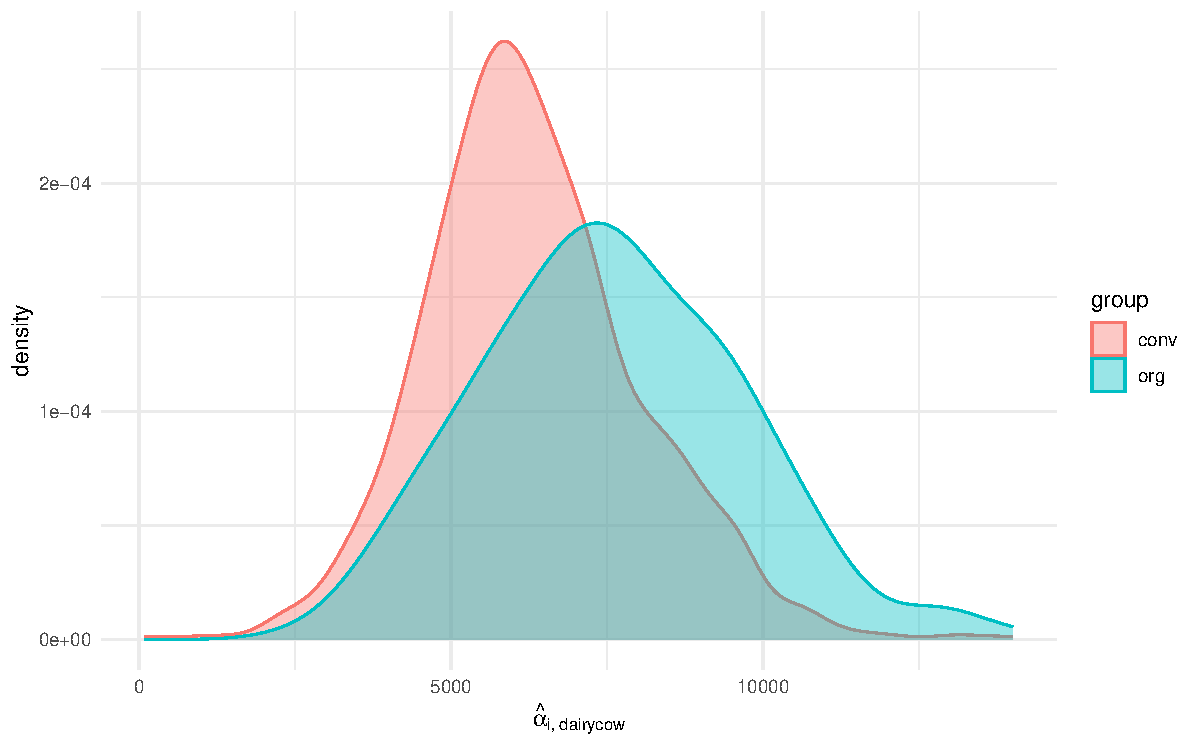
\includegraphics[width=0.83\textwidth]{pictures/coef_distrib_OK_107_PG_51.pdf}
\end{frame}

\begin{frame}[hvid]
\frametitle{\vspace{-3ex}Preliminary Results: Gamma for Milk Yield}
\vspace{-1ex}
\centering
\includegraphics[width=0.7\textwidth]{pictures/distrib_gamma_maelkeydelse.pdf}
\end{frame}

\begin{frame}[hvid]
\frametitle{\vspace{-3ex}Conclusion}
Preliminary Results
\begin{itemize}
%    \item Using an additional dairy cow in \textit{organic} milk production is probably associated with an increase in average labour costs of around 7578 kr.
%    \item Using an additional dairy cow in \textit{conventional} milk production is likely associated with an increase in average labour costs of around 6308 kr.
     \item On average, \textit{organic} farms spend about 7,578 kr. in labour per dairy cow, while \textit{conventional} farms spend about 6,308 kr. labour per cow.
     \item On average, a 1,000 kg higher milk yield per cow is associated with about 42 kr. higher labour cost per dairy cow.
\end{itemize}
\vspace{2ex}
Future Research
\begin{itemize}
    \item Explore the inclusion of disease prevalence variables (e.g., mastitis, ketosis, lameness, metritis and other cases of illness).
    \item Do the same analysis for veterinary costs (in addition to labour costs)
    \item Use panel data instead of cross-sectional data
\end{itemize}
\end{frame}

\end{document}